\documentclass[12pt]{article}
%\usepackage[utf8]{includeenc}
%\usepackage{draftwatermark}
%\SetWatermarkText{\textsc{Working Draft}}
%\SetWatermarkScale{0.6}
%\SetWatermarkColor[rgb]{1.0,0.33,0.33}
%\SetWatermarkLightness{0.93}
%\SetWatermarkAngle{55.789}

% All packages are defined in this file (e.g., Tikz, etc...)
%%novalidate

\usepackage{calc}
\usepackage{booktabs}

\usepackage[T1]{fontenc}
\usepackage{graphicx}
\usepackage{xcolor}
\usepackage{xspace}
\usepackage{comment}
\usepackage{float}
\usepackage{amssymb, amsmath}
\usepackage{kbordermatrix}
\usepackage{tikz}
\usepackage{lipsum}
\usepackage{listings}
\usepackage{minted}
\usepackage{comment}
\usepackage{wrapfig}
\usepackage{hyperref}
\usepackage{ragged2e}

\usepackage[backend=biber,style=numeric, sorting=none]{biblatex}
\addbibresource{references.bib}

\usetikzlibrary{arrows, calc, matrix, positioning, shapes.geometric}

\def\name{Elixxir\xspace}

\newcommand{\rn}[2]{%% "rn": "remember node"
    \tikz[remember picture,baseline=(#1.base)]\node [inner sep=0] (#1) {$#2$};%
}
\renewcommand{\kbldelim}{[}% Left delimiter
\renewcommand{\kbrdelim}{]}% Right delimiter


%%%%%%%%%%%%%%%%%%%%%%%%%%%%%%%%%% TIKZ SHAPES %%%%%%%%%%%%%%%%%%%%%%%%%%%%%%%%%%%%%

\tikzstyle{startstop} = [rectangle, rounded corners, minimum width=3cm, minimum height=1cm,text centered, draw=black, fill=red!30]

\tikzstyle{io} = [trapezium, trapezium left angle=70, trapezium right angle=110, minimum width=3cm, minimum height=1cm, text centered, draw=black, fill=blue!30]

\tikzstyle{process} = [rectangle, minimum width=2cm, minimum height=2cm, text centered, draw=black, fill=orange!30]

\tikzstyle{block} = [rectangle, minimum width=2cm, minimum height=1.5cm, text centered, draw=black, fill=orange!30]

\tikzstyle{decision} = [diamond, minimum width=3cm, minimum height=1cm, text centered, draw=black, fill=green!30]

\tikzstyle{arrow} = [thick,->,>=stealth]

%%%%%%%%%%%%%%%%%%%%%%%%%%%%%%%%%%%%%%%%%%%%%%%%%%%%%%%%%%%%%%%%%%%%%%%%%%%%%%%%%%%%%%


% colors
%\definecolor{color1}{HTML}{000060}
%\definecolor{color1}{HTML}{3667AB} -> MixxLabs
\definecolor{color1}{HTML}{090189}
%\definecolor{color1}{HTML}{8C260F}
%\definecolor{color2}{HTML}{333333}
\definecolor{color2}{HTML}{000000}

% fonts
\usepackage{fontspec}
\defaultfontfeatures{Mapping=tex-text}
\setmainfont
[ExternalLocation=fonts/,
BoldFont=Lato-Bold.ttf,
ItalicFont=Lato-Italic.ttf,
BoldItalicFont=Lato-BoldItalic.ttf]
{Lato-Regular.ttf}
\newfontfamily\headingfont[ExternalLocation=fonts/,ItalicFont=Lato-BlackItalic.ttf]{Lato-Black.ttf}
%%%

% Page Settings
\usepackage{geometry}
\geometry{a4paper,
hmargin=1in,vmargin=1in,
head=0.5in,foot=0.5in}

% hbox controls
\pretolerance=150
\tolerance=100
\setlength{\emergencystretch}{3em}

% Line, paragraph, list, etc spacing
\setlength{\parindent}{0em}
\setlength{\parskip}{0.75em}
\linespread{1.1}
\usepackage{enumitem}
\setlist{nolistsep}




\usepackage[hang]{caption}
\DeclareCaptionFormat{upper}{#1#2\makeatletter{#3}\par}
\captionsetup{labelfont={bf,color=color2},textfont={normalsize,color=color2},format = upper,figurename=Figure,tablename=Table}

%%% fancy sections
\usepackage{titlesec}
%\titleformat{\chapter}{\headingfont\LARGE\bfseries\scshape\color{color1}}{\thechapter}{1em}{}[\titlerule]
\titleformat{\section}{\color{color1}\headingfont\Large\bfseries\uppercase}{\thesection}{1em}{}[\titlerule]
\titlespacing{\section}{0pt}{*1}{*1}

\titleformat{\subsection}{\color{color1}\headingfont\large\bfseries\uppercase}{\thesubsection}{1em}{}
\titlespacing{\subsection}{0pt}{*0}{*0}


\titleformat{\subsubsection}{\color{color1}\headingfont\bfseries\uppercase}{\thesubsubsection}{1em}{}
\titlespacing{\subsubsection}{0pt}{*0}{*0}

%%%

% head and foot
\usepackage{fancyhdr}
\pagestyle{fancy}
\lhead{}
\chead{}
\makeatletter
\rhead{\color{color2}\@date}
\makeatother
\newlength{\myheight}
\lfoot{
\settoheight{\myheight}{\thepage}
\raisebox{-2ex-0.5\myheight}{
\includegraphics[height=4ex]{img/elixxirLogo.pdf}}
}
\cfoot{\color{color2} \name Technical Brief}
\rfoot{\color{color2}\thepage}
\renewcommand\headrulewidth{0pt}
\renewcommand\footrulewidth{0pt}

% custom titlepage
\makeatletter
\newcommand*\DefVar[1]{\@namedef{#1}##1{\global\@namedef{get#1}{##1}}}
\DefVar{summary}
\renewcommand{\maketitle}{
\vspace*{\fill}
\begingroup

\begin{center}


\includegraphics[width=\textwidth]{img/elixxirLogo.pdf}


\begin{tikzpicture}
    \node[draw=none,%color1,line width=0.4pt,
      fill=color1,
      inner sep = 10pt,
      text width=\textwidth-20pt,
      text centered
    ] {\color{white}\headingfont\bfseries\huge\@title};
\end{tikzpicture}

\bigbreak \bigbreak \bigbreak 

\LARGE \textbf{Technical Brief}

\bigbreak \bigbreak \bigbreak 
\headingfont\bfseries\large\@author\par
{\normalfont\normalsize\textbf{Version:} 0.7}
\bigbreak \bigbreak \bigbreak 
\bigbreak \bigbreak \bigbreak 
\bigbreak \bigbreak \bigbreak 


\iffalse
\bigskip\medskip
{\color{color2}\normalfont\normalsize\textbf{Summary:}\\
\getsummary}
\fi
\end{center}
\endgroup
\vspace*{\fill}
\clearpage
}
\makeatother
%%%

%%% fancy boxes
\usepackage{tcolorbox}
\usepackage{wrapfig}
\def\fullboxbegin{
\bigskip
\begin{tcolorbox}[colback=color1,colframe=color1,coltext=white,arc=0mm,boxrule=0pt]
}
\def\fullboxend{\end{tcolorbox}\medskip}
%
\def\leftboxbegin{
\begin{wrapfigure}{l}{0.5\textwidth}
\begin{tcolorbox}[colback=color1,colframe=color1,coltext=white,arc=0mm,boxrule=0pt]
}
\def\leftboxend{
\end{tcolorbox}
\end{wrapfigure}
}
%
\def\rightboxbegin{
\begin{wrapfigure}{r}{0.5\textwidth}
\begin{tcolorbox}[colback=color1,colframe=color1,coltext=white,arc=0mm,boxrule=0pt]
}
\def\rightboxend{
\end{tcolorbox}
\end{wrapfigure}
}
%
\newcounter{frames}
\def\frameboxbegin#1{
\bigskip
\refstepcounter{frames}
\begin{tcolorbox}[colback=white,colframe=color1,arc=0mm,title={\MakeUppercase{\textbf{Note \arabic{frames}}: #1}}]
}
\def\frameboxend{
\end{tcolorbox}
}
%%%


% Images used throughout the document (e.g., system architecture, etc) are included in the folder img, if you use tikz icons put them in an icons folder
% All sections are outsourced from the sections folder

%%% NOTICE %%%
% Per our discussion, we're limiting ourselves to the core technical meat and not all of the extensions so as not to overload readers and muddy the water. 
% Remember, we want this to be accessible to the public! That means not going crazy with the detail and instead focusing on explaining why, in simple language, things work. To that end, we're only talking about the sections listed below, and that explicitly means limited discussion of the following (with exceptions listed):
% 1. Token Economics, but mentioning block reward/generation is OK
% 2. Governance (including node election and stake), except to mention it exists, also OK to mention voting protocol RSV/Scantegrity/etc
% 3. 2-phase payments---yes the single phase is only secure in the context of the larger platform, but 2-phase is 2-complicated.
% 4. Any of the anonymous large payload designs -- completely off-limits
% 5. dApp details, except to acknowledge you can build them
% 6. Private user discovery protocol -- completely off-limits
% 7. Linked coins protocol -- completely off-limits
% 8. Group and Channel messaging protocols -- completely off-limits
% 9. The anonymous & decentralized credentialing systems -- completely off-limits
% 10. Any of the state of the tech, although listing or screenshotting something might be ok... talk to me first
% 11 (yes, of course i made this one up to make the list count prime -- deal with it :-D). Any of the half-baked stuff we've been kicking around (the SGX matryoshka replacement idea, cmix w/ xors extension, etc) -- completely off-limits
%
% Remember, the plan is to release the core tech, gather feedback and hopefully get people who can contribute interested. Ultimately, we do want a community formed around this, and we are trying to set a high bar of clear and accessible technical comms. I know this is frustrating to some, but we do not have the resources to write up everything to this standard as quickly as we need to, and we will release the details of the other topics either in the whitepaper or in due time. 
%
% If you have problems/questions/concerns/ideas, please bring them up with me (Rick) and we will address 1-on-1 before going to the group.
%% END NOTICE %%


%%%%%%%%%%%%%%%%%%%%%%%%%%%%%%%%%% TITLE PAGE %%%%%%%%%%%%%%%%%%%%%%%%%%%%%%%%%%%%%

\title{Scalable Digital Sovereignty}

\author{www.elixxir.io}

\date{\today}

\begin{document}

\maketitle

% executive summary
\section*{Executive Summary}

For blockchain technology and digital currencies to achieve mainstream adoption, consumers require a scalable, high-performing messaging and payment platform that affirms and preserves a user's right to digital sovereignty, without compromising user experience---blockchain performance and convenience. The \name blockchain has been designed to address performance issues hindering the adoption of current decentralized systems, while maintaining the privacy consumers require.

\name provides users with:
\begin{itemize}
    \item \textbf{Speed}: Payment completion and message transmission are completed in a matter of seconds.
    \item \textbf{Transactional privacy}: Only senders and receivers can review and prove payment history. Transaction data is not stored on the blockchain.
    \item \textbf{Communication privacy}: The identity of communicating parties and their devices remains private.
\end{itemize}

The architecture of the \name platform provides users with performance that scales linearly as computers join the network. Network nodes are incentivized to maximize throughput while ensuring security, and payments use a faster hash-based ownership mechanism instead of digital signatures. 

The \name consensus requires nodes work in teams that are sequentially assigned the task of generating blocks as opposed to requiring all nodes to compete individually. Within teams, all nodes are required to independently create cryptographically verifiable proofs that are published alongside the new block, proving that transactions were received and processed properly. \name users are able to validate the integrity of transaction processing using these proofs. Additionally, the existence of just one honest node within the team is sufficient to preserve the anonymity of users. 

\name's privacy features are unique and novel capabilities in decentralized technology. Both users and distributed applications enjoy the benefits of a sophisticated anonymization protocol that enables private messaging and transactions. The platform does not store transactions on the blockchain, only tokens, further protecting user privacy.

The team behind the creation of \name is comprised of pioneers of practical, anonymous and verifiable cryptographic systems. Its members are among the first to propose and deploy digital currencies, mix networks, unpermissioned cryptography, anonymous user discovery, verifiable voting systems, and many other advances in cryptography. They have dedicated their collective decades of experience in this space to this breakthrough platform. 

\name is capable of replacing current centralized systems at scale and with quick response times. The \name platform targets game-changing verifiability, privacy, and digital sovereignty because, together, they are the digital future.


% letterFromDavid
\section*{A Letter from our Founder}

\footnotesize

``Large-scale automated transaction systems are imminent. As the initial choice for their architecture gathers economic and social momentum, it becomes increasingly difficult to reverse. Whichever approach prevails, it will likely have a profound and enduring impact on economic freedom, democracy, and our informational rights.''

``Restrictions on economic freedom may be furthered under the current approach. Markets are often manipulable by parties with special access to information about other participants' transactions. Information service providers and other major interests, for example, could retain control over various information and media distribution channels while synergistically consolidating their position with sophisticated marketing techniques that rely on gathering far-reaching information about consumers. Computerization has already allowed these and other organizations to grow to unprecedented size and influence; if computerization is continued along current lines, such domination might be further increased. But the computerization of information gathering and dissemination need not lead to centralization: integrating the payment system presented here with communication systems can give individuals and small organizations equal and unrestricted access to information distribution channels. Moreover, when information about the transactions of individuals and organizations is partitioned into separate, unlinkable relationships, the trend toward large-scale gathering of such information, with its potential for manipulation and domination of markets, can be reversed.''

``Attempts to computerize under the current approach threaten democracy as well. They are, as mentioned, likely to engender widespread opposition; the resulting stalemate would yield security mechanisms incapable of providing adequate prior restraint, thus requiring heavy surveillance, based on record-linking, for security. This surveillance might significantly chill individual participation and expression in group and public life. The inadequate security and the accumulation of personally identifiable records, moreover, pose national vulnerabilities. Additionally, the same sophisticated data acquisition and analysis techniques used in marketing are being applied to manipulating public opinion and elections as well. The opportunity exists, however, not only to reverse all these trends, by providing acceptable security without increased surveillance, but also to strengthen democracy. Voting, polling, and surveys, for example, could be conveniently conducted via the new systems; respondents could show relevant credentials pseudonymously, and centralized coordination would not be needed.''

``The new approach provides a practical basis for two new informational human rights that is unobtainable under the current approach. One is the right of individuals to parity with organizations in transaction system use. This is established in practice by individuals' parity in protecting themselves against abuses, resolving disputes, conferring proxy, and offering services. The other is the right of individuals to disclose only the minimum information necessary: in accessing information sources and distribution channels, in transactions with organizations, and---more fundamentally---in all the interactions that comprise an individual's informational life.''

``Advances in information technology have always been accompanied by major changes in society: the transition from tribal to larger hierarchical forms, for example, was accompanied by written language, and printing technology helped to foster the emergence of large-scale democracies. Coupling computers with telecommunications creates what has been called the ultimate medium---it is certainly a big step up from paper. One might then ask: To what forms of society could this new technology lead? The two approaches appear to hold quite different answers.''


\begin{flushright}
    --- David Chaum \\ 1987~\cite{Chaum85}
\end{flushright}

\normalsize

\setlength{\parskip}{0em}
\tableofcontents
\setlength{\parskip}{0.75em}

\break

% High-Level Overview
\section{Introduction}

\name is a decentralized blockchain platform that allows users to communicate and exchange value securely and confidentially. \name's breakthrough design produces a decentralized network capable of potentially scaling to process transactions on a mega-tps scale, far exceeding the kilo-tps scale characteristic of conventional mainstream payment systems. The \name design provides users with a blockchain platform that achieves the kind of performance that consumers expect from current centralized systems:

\begin{enumerate}
    \item \textbf{Speed}: Payment processing on the order of seconds, from start to irrevocable finality.
    \item \textbf{Scale}: Tens of thousands of transactions per second.
    \item \textbf{True Privacy}: Transactions that are not linked to users or to other transactions. Communications are end-to-end encrypted, they can only be read by the intended recipients.
\end{enumerate}

\name has been designed to realize the vision of a world in which digital sovereignty truly exists, a world in which users can protect themselves and control their privacy by revealing only the absolute minimum amount of information necessary to conduct transactions. \name has been built for the user. Users generate and control their own keys. Users control access to all of their confidential interactions. Users have exclusive access to all their digital property. Users control linkage of any personal credentials to their data. Users are in control of their digital future.

Mainstream adoption of blockchain technology requires a platform capable of scaling to process the necessary high transaction volumes while protecting user's digital sovereignty. To that end, the \name team---led by Dr. David Chaum---has leveraged their experience as innovators in  blockchain technology, consensus mechanisms, unpermissioned cryptography, cryptocurrencies, and online voting to address this challenge through the creation of \name.



% System Architecture or System Overview
\section{Architecture Overview}
\label{section:architecture}

\begin{wrapfigure}{r}{0.36\textwidth}
    \centering
    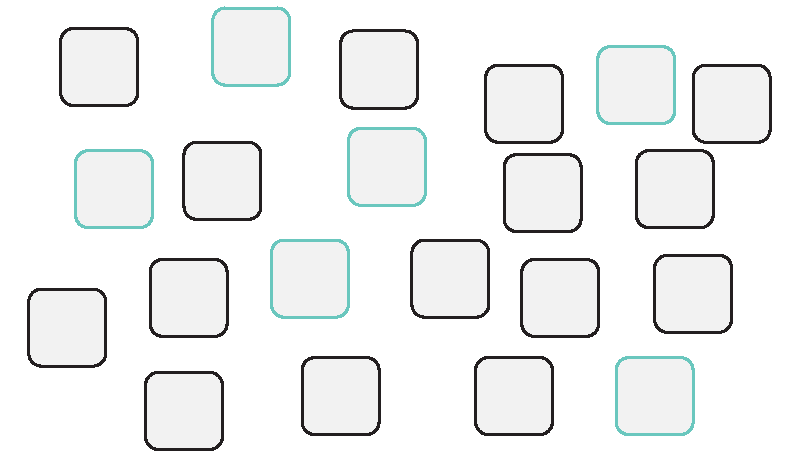
\includegraphics[width=0.35\textwidth]{img/cohort.pdf}
    \caption{A single team (in teal), randomly selected from a group of nodes.}
    \label{fig:team}
\end{wrapfigure}

In order to protect a user's digital sovereignty, the \name protocol utilizes accelerated mix networks to ensure confidentiality. A mix network~\cite{mix_81} is a routing protocol that uses cryptography to dissociate the origin, contents, and destination of a message. A ``message'' in this context could be simply a text message, or else a payment transaction on a blockchain. The \name protocol uses mix networks in combination with a distributed ledger to create a confidential blockchain. 

Unlike other blockchain protocols, in the \name protocol, groups of nodes are deterministically organized into teams. \name teams are temporary, and exist only for the duration of the block they are responsible for generating. The team uses a consensus protocol, explained in Section~\ref{section:consensus}, to validate and authenticate operations that anonymize each encrypted message, independently agree to process all messages before decryption, and then independently decrypt~\footnote{Messages are still end-to-end encrypted over the network.} and process each message. Following block generation, the team disbands and member nodes become available to be placed on a new random team. As shown in Figure~\ref{figure:simple-architecture}, the team allows messages to be sent both directions with anonymity. 

\begin{wrapfigure}{L}{0.58\textwidth}
    \centering
    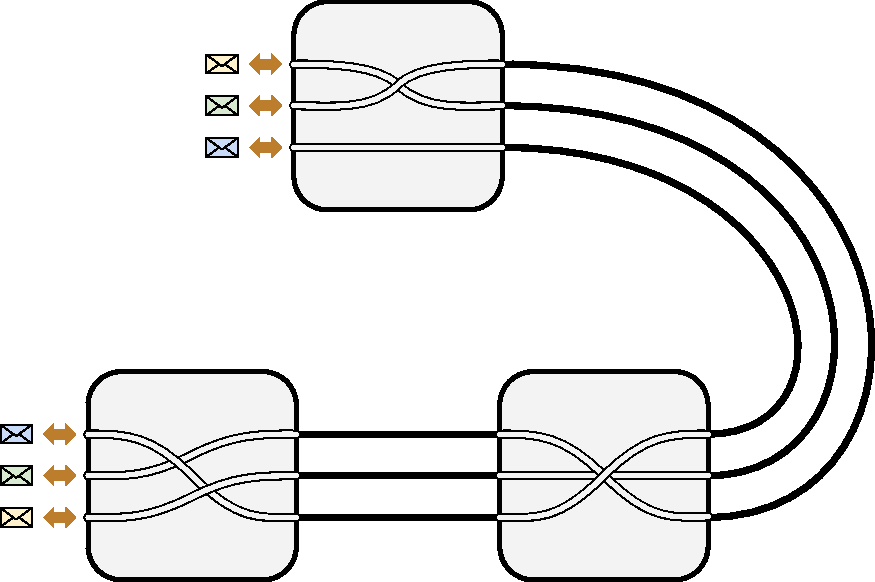
\includegraphics[width=0.5\textwidth]{img/Simple-Architecture.pdf}
    \caption{Each team creates an anonymous, verifiable, bi-directional transaction channel to process each block in the blockchain.}
    \label{figure:simple-architecture}
\end{wrapfigure}

All operations conducted by \name teams are accelerated through the use of precomputation~\cite{precomps}. These precomputations produce a template that dictates how the nodes within a team must process information during block generation. Consequently, the template is completely defined before any message information arrives for block generation. The use of precomputation ensures confidentiality while dramatically increasing the speed at which information can be processed to generate a block.

Nodes must be elected to participate in processing the messages and transactions on the \name network. In order to be eligible for election, a node is required to stake tokens on the network. Once elected, a node is eligible to be placed into an \name team. 

\begin{figure}[H]
    \centering
    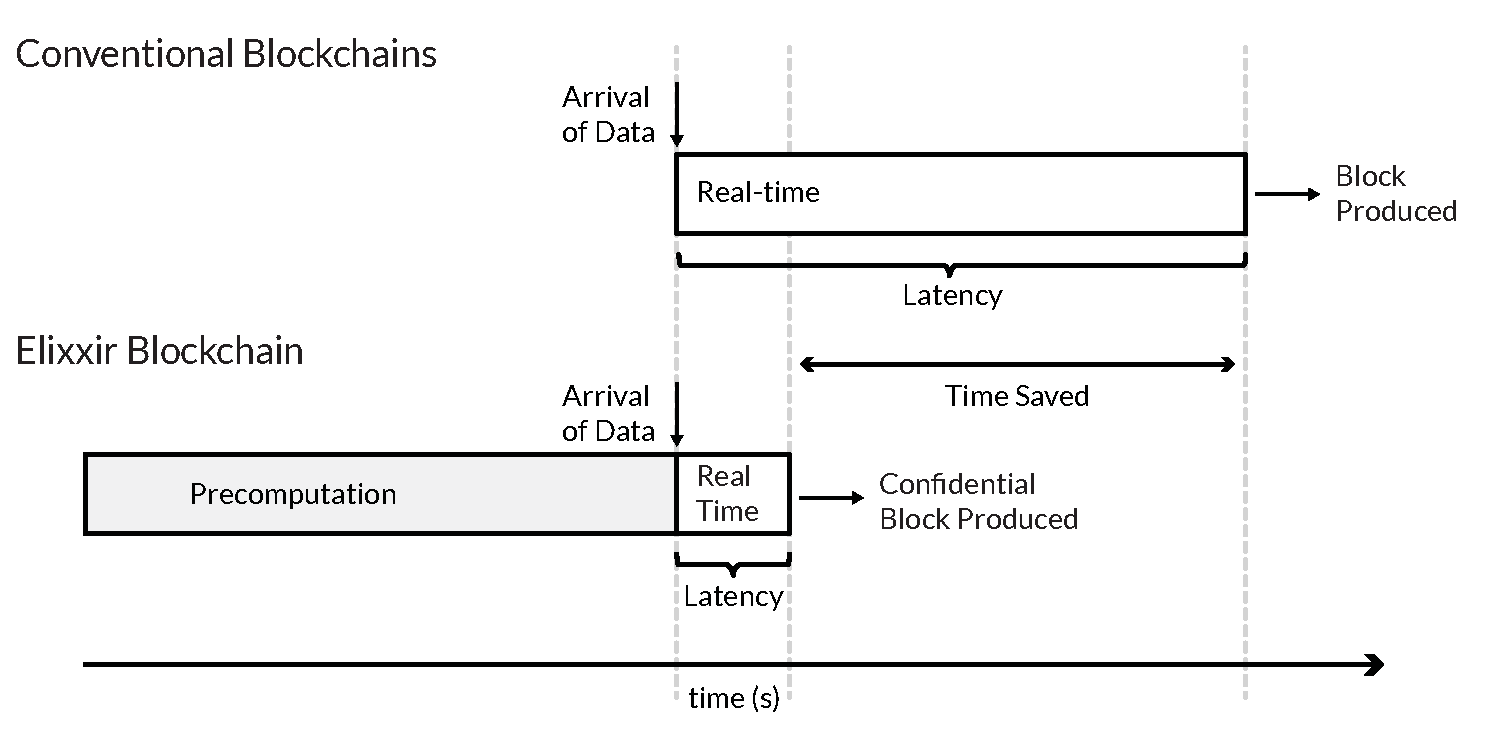
\includegraphics[width=\textwidth]{img/Processing.pdf}
    \caption{Time-consuming, computationally-intensive team precomputation is performed before transactions are sent or received. This allows very fast real-time computation of transactions to generate each block in the blockchain. The use of precomputation decouples security from latency as seen in conventional blockchains, delivering a greater level of security without the latency penalty.}
    \label{figure:processing}
\end{figure}

There are two phases involved in block production by an \name team as depicted in Figure~\ref{figure:processing}. First, the team performs a computationally-intensive precomputation as discussed above, producing a unique template defining how the information or messages of the block will be processed. When messages arrive, the nodes of the team work together to process the messages in real time according to this unique template, a process that takes less than 1/20th of the precomputation time. 

Unlike sharding proposals or the lightning network~\cite{lightning}, \name teams cannot influence the consensus mechanism's integrity as all aspects of block production are independently predetermined in a strict, verifiable, and immutable manner. Additionally, all nodes in a team independently provide proofs that validate the block prior to final block confirmation. 

To ensure proper system functionality, nodes collectively and independently generate cryptographic proofs as commits of batch integrity prior to decryption. In the event that commits do not match, all proofs produced by the nodes can be inspected to identify node failure or malfeasance. Once a malicious or malfunctioning node has been identified, honest nodes refuse further contact and broadcast proof of malfeasance or malfunction to the rest of the network. If a node is verified to be malicious, it loses its stake of tokens, which are burned, and the node is ejected from the network.  These, and additional security mechanisms, allow users to prove incorrect handling of their transaction, while rendering them unable to accuse the nodes or the team falsely.

\subsection{Scaling Strategy}

At any given time, tens to hundreds of teams will exist within the network in varying stages of precomputation. However, at any given time, only one team will be producing a block. These precomputations overlap in a cascade, as shown in Figure~\ref{figure:processing-cascade}. Consequently, the throughput of the network increases with the addition of more nodes to the network forming more teams. This allows the platform to linearly scale its capacity with the addition of more nodes.

\begin{figure}[H]
    \centering
    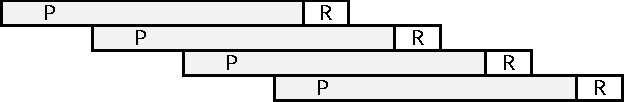
\includegraphics[width=\textwidth]{img/Processing-Cascade.pdf}
    \caption{Teams are organized into a cascade pipeline to maximize the number of transactions that can be processed by our platform.}
    \label{figure:processing-cascade}
\end{figure}

Increasing the number of teams results in increased network resilience as more teams must be brought down to impair or completely disrupt the network. As longer precomputation times become feasible, the number of messages processed by each team can also be increased. 

\subsection{Block Propagation}

Once generated, block data is broadcast to each node in the next team. Once the next active team has received the block data, data is then broadcast to the rest of the nodes in the network. This sequence prioritizes communication to the next team responsible for block generation, ensuring efficient block propagation.


% Consensus
\section{Consensus Protocol}
\label{section:consensus}

The \name consensus protocol is designed to facilitate a blockchain messaging and payment solution that is anonymous and capable of scaling. The \name consensus protocol enables the creation of a resilient, trustless platform that is capable of meeting the diverse array of applications envisioned for the blockchain.

Each node in the team performs the following operations in the \name consensus protocol:

\begin{enumerate}
    \item Before any transactions are known, the team defines a template comprising commits to message slots for transactions. The template determines, but does not reveal, the order in which each transaction will be processed within the block, and how the transactions will be opened by nodes in the team.
    \item Independently, the nodes within the team agree and commit to the transactions without knowing the content of the transactions, and broadcast that commitment to all other team nodes. 
    \item As a team, the nodes open all transactions together in the predetermined order, revealing their contents. When the team agrees that all transactions are valid, and commits have been made to processing the transactions properly, nodes again broadcast these commits to all other nodes.
    \item The team then executes all transactions. Each node independently generates and broadcasts a block that must be identical to the block produced by all other nodes in the team.
\end{enumerate}

The \name consensus has the advantage over other consensus mechanisms in that each node participating in the team provides a short proof that it processed the transactions properly, and publishes that proof as part of the block. Additionally, each team commits to each stage of the block’s production before the contents of the block are known. As a result, the output block is a product of the validated input. Any disagreement results in an incorrect proof being attributed to the misbehaving node, which disables that node identity in the network.

\subsection{Consensus Properties}

\begin{figure}[ht]
    \centering
    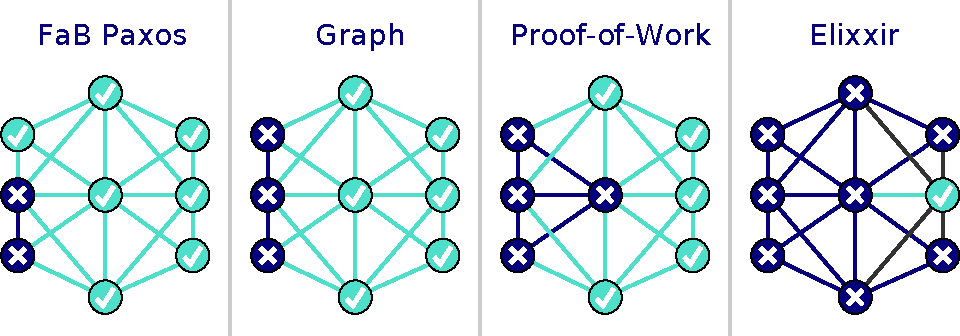
\includegraphics[width=\textwidth]{img/Consensus.pdf}
    \caption{The number of honest (green) nodes, hashrate units, or stakes required to achieve consensus in a 9-unit configuration. Unlike graph and traditional proof-of-work (and -stake) solutions, \name consensus requires only a single honest node to perform user-verifiable operations.}
    \label{figure:consensus}
\end{figure}

Unlike other platforms, consensus in \name is not vulnerable to a 51\% attack, as illustrated in Figure~\ref{figure:consensus}. Any single honest node protects team consensus. An entirely dishonest team can only produce proofs for the transactions submitted by the set of users in that round. As such, nodes cannot create fake transactions to their own benefit, nor valid proofs for forged transactions. A completely dishonest team---an unlikely event---is limited to only being able to change the order of transactions, de-anonymizing the transactions, or failing to provide a proof, i.e., faking a failure.

Consensus algorithms in the blockchain space have been primarily hampered by bandwidth limitations; blocks must be propagated to a majority of the system before finality is realized. Even a small block requires exponentially more bandwidth than its file-size to transfer across a network. In the \name consensus protocol, nodes reach finality by evaluating short proofs that are propagated optimally through the network. As a result, the \name consensus mechanism facilitates seconds-long finality times.

\subsection{Team Resilience}

The \name protocol has a built in timeout period. A team’s failure to complete a block by the timeout period requires clients to resubmit their transactions to another team for processing. For this delay, the failing team does not receive any token revenue for computational work. Team nodes may face further repercussions, such as failing to be re-elected to the network, as failure metrics are publicly available. The potential penalties incentivize nodes to provide resilient network connectivity to ensure that teams they participate in complete block generation. Attackers are dissuaded as well because the teams are constantly moving, unpredictable targets, forcing asymmetric attack patterns to affect network stability. 

As network team size increases, the probability of a node impacting completion of a block increases, so the primary engineering trade-off for resilient block generation is the size of the teams. Also, as team sizes grow, the real-time processing times increase and throughput decreases. Team sizes should range from 5 to 30 nodes to produce a system that exhibits seconds-long block generation. Such team sizes compare favorably with the entirety of the controlling interest\footnote{For example, 21 nodes control the EOS network, and ~5 mining pools control Bitcoin. (\url{https://www.ccn.com/bitmains-mining-pools-now-control-nearly-51-percent-of-the-bitcoin-hashrate/})} in other networks.

\subsection{Network Resilience}

The \name platform has been designed to incentivize nodes to follow the rules of the protocol. Failure to do so results in penalties for all nodes in teams containing malicious or unproductive nodes. Nodes are incentivized to allow the protocol to operate without interference. The protocol also offers significant flexibility when dealing with network failures. The set of valid nodes is known, as they must have been elected to join the network. Since the teams are arranged in a cascade, the failure of any one team can be readily mitigated by the next team in the cascade.

Successfully interrupting block generation would require all scheduled teams to be disabled. The most common failures---individual node failures, geographical outages, an entire country being taken offline, etc.---are handled without affecting platform operation. When a targeted, extended, large-scale network attack does successfully disable all scheduled teams, the platform is capable of supporting the same recovery mechanisms found in other systems, like “longest chain/most computation wins”.

\subsection{Participatory equality}

The egalitarian properties achieved by \name compare exceptionally favorably to other consensus mechanisms. Specifically, the greater computational capability or larger stake of a node does not advantage that node over others in this platform.

The successful completion of a block is a cryptographically secured group computation analogous to a proof of useful work. One can think of processing the transactions as a mining operation where the work is not wasted, but directly corresponds to providing the properties of the platform. Hence, any unforeseen algorithmic advances, new ASIC designs, or other developments do not advantage one team or node over another. Additionally, each node is treated equally and each one automatically audits the fidelity of all other nodes.

\subsection{Sybil attack resistance}
Within the \name protocol, sybil attack \cite{sybil} resistance is created through the use of verifiable real-time inter-node performance testing, staking, and elections. \textit{Staking} requires nodes to place a governance-determined number of tokens in an “escrow” that will be burned if they are expelled from the system for malfeasance.

\textit{Elections} in \name utilize methodologies such as random sample voting~\cite{rsv} and decoy balloting for honest and trustworthy elections by which users of the system can elect which nodes are verified to join teams, and which can be excluded. All elections in the \name platform will use cryptographically secured, voter-verifiable, end-to-end election protocols. The \name team has pioneered these protocols, being the first to propose such systems~\cite{unconditionalsecretballots}, the first to deploy them in a binding governmental election~\cite{takomapark}, and the first to use a blockchain for publishing election data in an election~\cite{commitcoin}.



% Payments
\section{Payments}
\label{section:payments}

\begin{figure}[H]
    \centering
    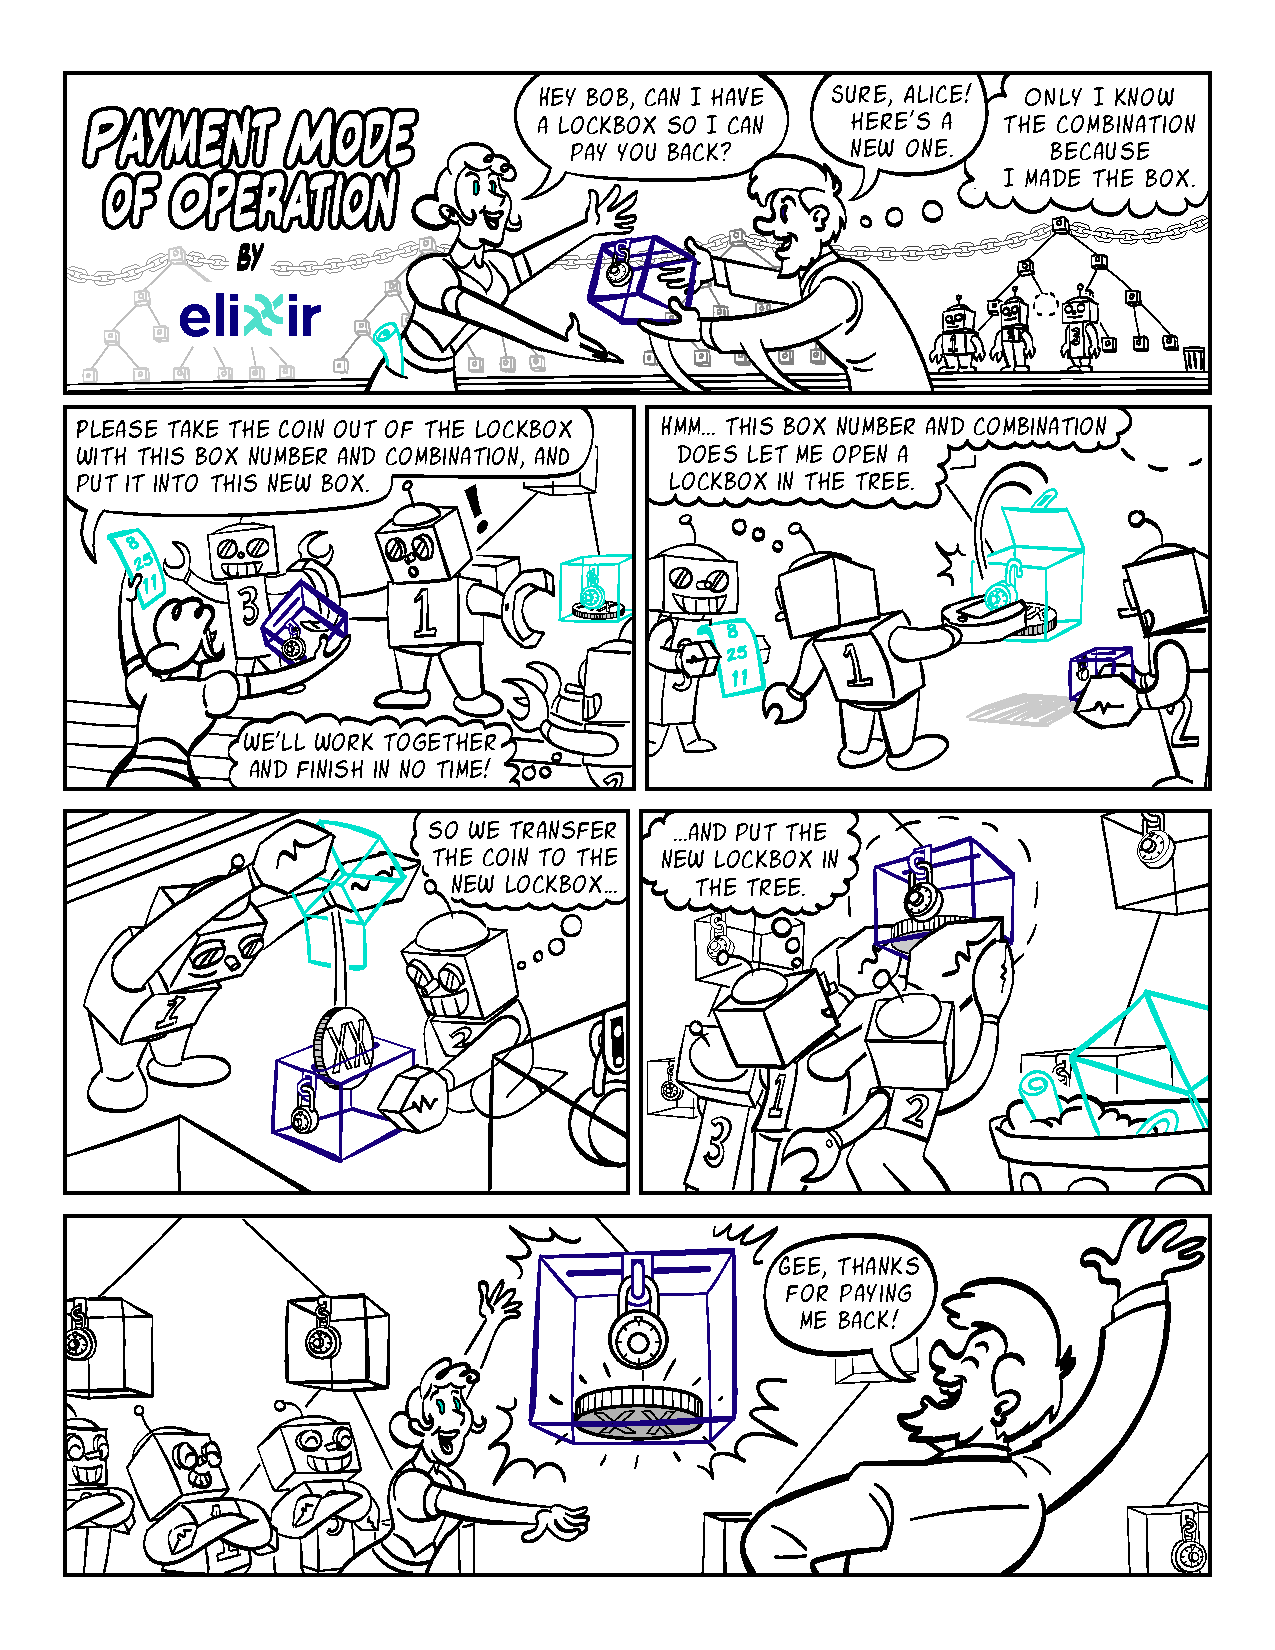
\includegraphics[width=\textwidth]{cartoons/PaymentOperation.pdf}
    %\caption{Illustration of an example transaction from Alice to Bob}
    %\label{fig:payment_cartoon}
\end{figure}

\break

Token handling in the \name platform has some unique attributes. Token handling in most conventional blockchain systems today is wallet-based. In the \name protocol, token handling is token based, meaning the token remains static, while a secret is required to prove ownership. These secrets are kept off-chain and change when ownership of a token is assigned to a new owner. 

\name secures individual tokens rather than securing an entire wallet as a whole. Each token owned by a user is secured through knowledge of an individual secret, which means that even if an attacker successfully performs a brute-force attack, only one single token from the user can be compromised.

\name blocks do not contain any information about transactions, i.e. sender, receiver, and amount. Instead, a block from the \name blockchain contains assignments of tokens to addresses belonging to the payee, and previous addresses belonging to the payer. Moreover, there is no information linking payer and payee in the blockchain, which translates into on-chain unlinkability. 

\subsection{Block Structure}

\name takes a new approach to the information contained in blocks. Each block contains nothing more than unordered lists of the past and new addresses to which tokens were assigned by the transactions of that block.

By analyzing the entire blockchain, an observer is unable to link the transacting parties or the features of the transaction to one another (i.e., how many were sent).  As a result, one can only infer that in a specific block a set of tokens have been unlinkably assigned to new addresses from old addresses.

To contextualize such block information, we show a snippet of what is present in the \name block explorer tool in Figure~\ref{fig:block_explorer}.

\begin{figure}[H]
    \centering
    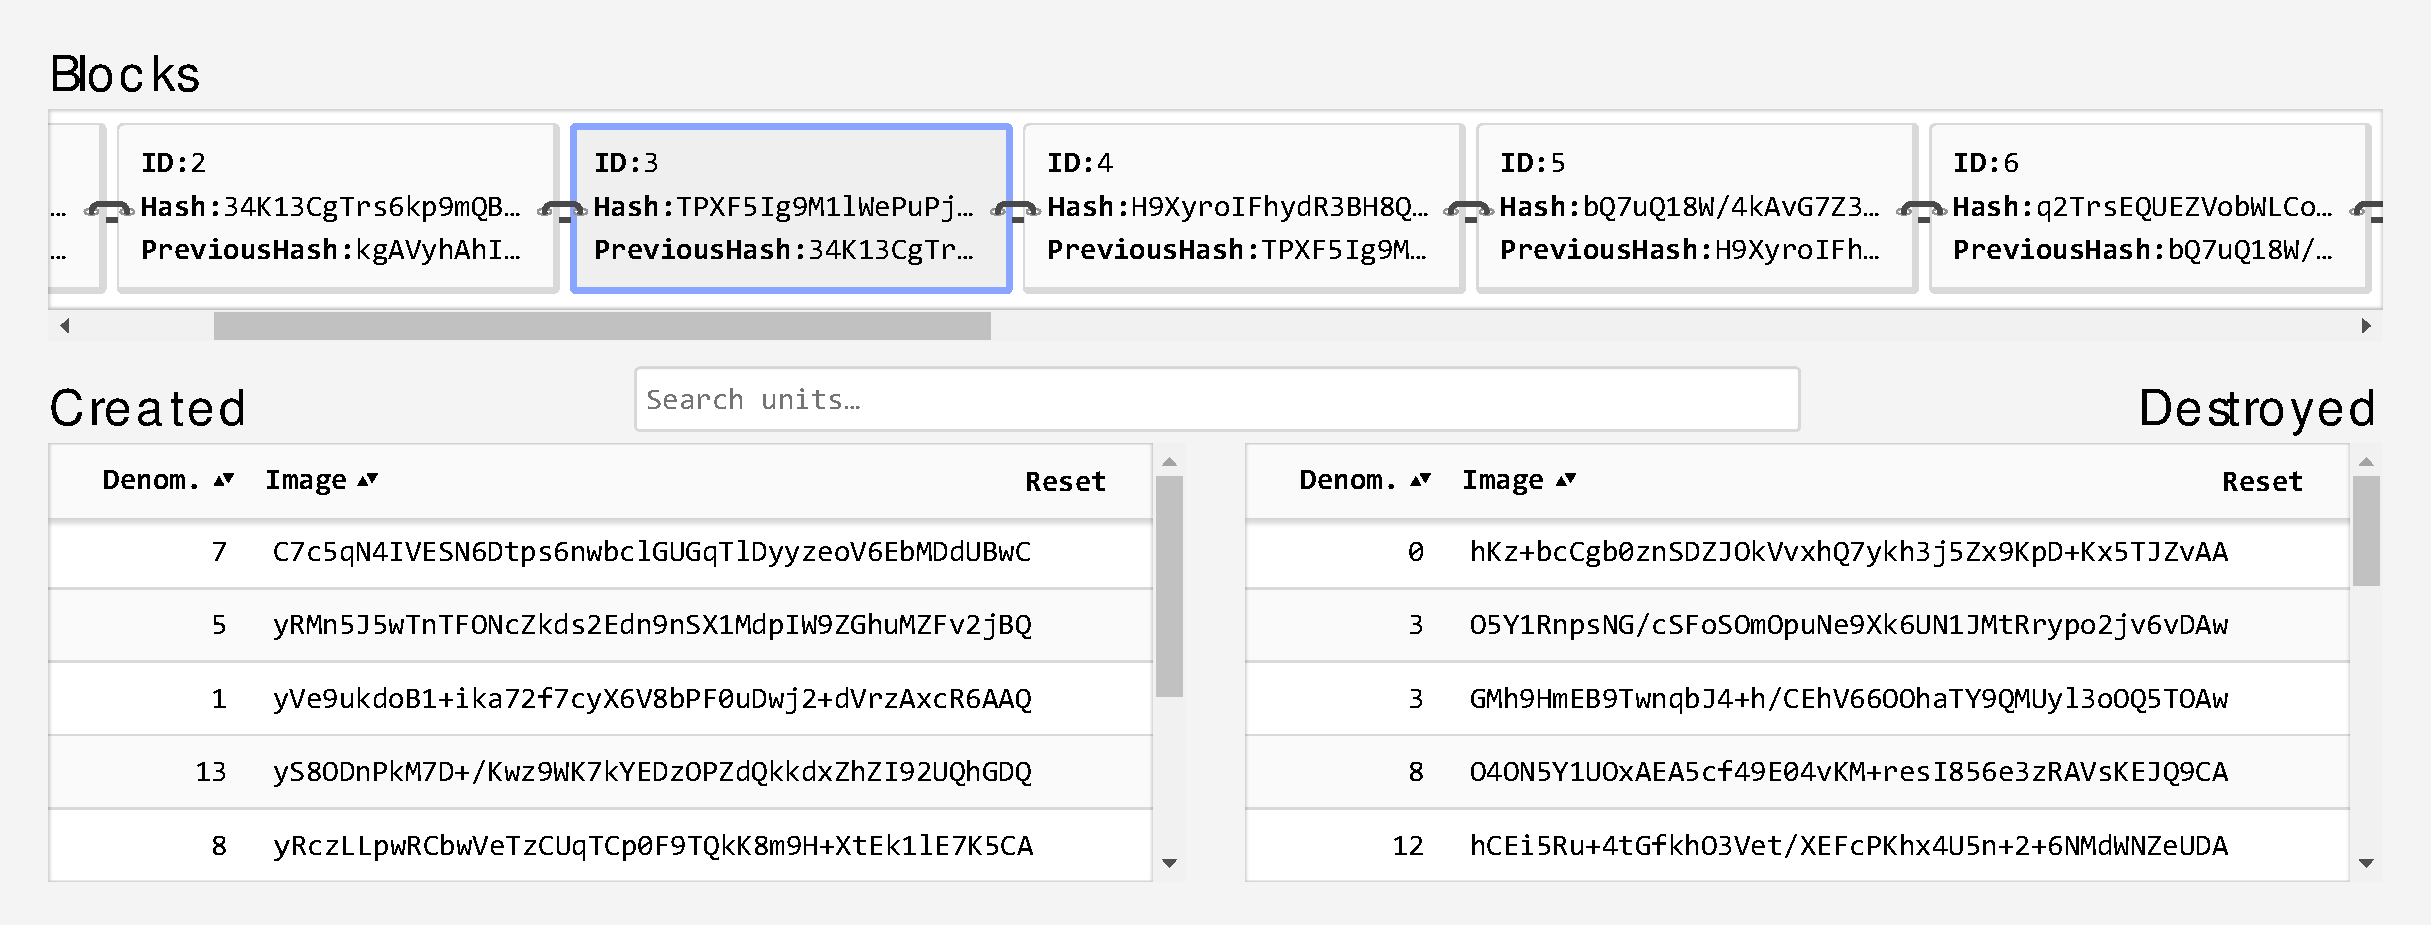
\includegraphics[width=\textwidth]{img/Block-Explorer.pdf}
    \caption{Block \#3 from the \name Block Explorer}
    \label{fig:block_explorer}
\end{figure}

Within both the block and the nodes, data is stored as a binary radix tree combined with a Merkle tree~\cite{merkle}. This structure allows for fast searching and rehashing of the root within the nodes, and for proofs to be generated that verify the existence of a token within a block. This is achieved simply by revealing the hashes of the block root, the token, and all non-leaf data blocks in between. As a result, shorthand proofs can be generated and used for validation in lieu of requiring all of the data of a relevant block referencing the transaction of interest. 

\subsection{Payment Preliminaries}

Normally, in the blockchain space, users submit a transaction---signed with their corresponding private key---to the system. The nodes in the system then check the validity of the transaction by employing the user's corresponding public key. If the key is valid and the user has funds to perform the payment, then the transaction is written to a block. 

\name introduces a new and faster concept: \textit{Hash-Based Ownership}. Since hash functions are considered infeasible to invert, users can use pre-images as proof of their ownership of specific images. By chaining this process of revealing these pre-images with our \name protocol, users are able to perform payment transactions anonymously and securely. Furthermore, this process ensures that no one is able to forge a fake transaction in an attempt to steal someone's tokens.

\subsection{Making a payment}

A simplified payment transaction in the system starts with an invoice. Bob sends Alice an invoice containing the destination address (where she should send the money). This address is an image (the output of a hash function) that Bob previously generated from a random preimage (a secret that is the input to a hash function).
    
Alice, after receiving the destination image (address), submits a payment transaction to the system. This transaction contains the preimage (secret) of a token she owns along with the image (address) from Bob's invoice.
    
The system checks whether the preimage (secret) Alice sent is valid and exists in the ledger and then transfers the specified amount from Alice's token to Bob's destination image (address). After processing the transaction successfully, the system returns a proof receipt to Alice that she can share with Bob, which validates that the transaction executed correctly.

This receipt provides proof that the transaction is properly recorded in the block by providing the Merkle path within the block of those tokens. This alone is enough proof that the transfer took place correctly and that, therefore, the tokens now belong to Bob. However, both parties (Alice or Bob) can freely check the blockchain and verify that the destination image (address) and the proper amount are present in the corresponding block.

\name's unique architecture and payment processing mechanisms offer three advantages over traditional approaches:

\begin{enumerate}
    \item User confidentiality is protected by the limited information that is available on-chain. 
    \item Security is increased substantially by securing tokens instead of wallets. In the exceptionally rare event that a successful brute-force attack does occur, security of at most one token may be affected. 
    \item Transaction processing is faster because hash-based ownership can be completed in a fraction of the time required for a digital signature in traditional blockchain platforms. 
 \end{enumerate}  
    
As others have said~\cite{sphincs}, when contrasting digital signatures characteristic of traditional blockchain platforms to hash-based digital signatures used in the \name platform, ``\textit{Every signature scheme uses a cryptographic hash function; hash-based signatures use nothing else}''  Lastly, unlike digital signatures, hashes are secure against quantum-computational capabilities.




% Message Mixing
\section{Mixing Messages and Transactions}
\label{section:mixing}

\begin{figure}[H]
    \centering
    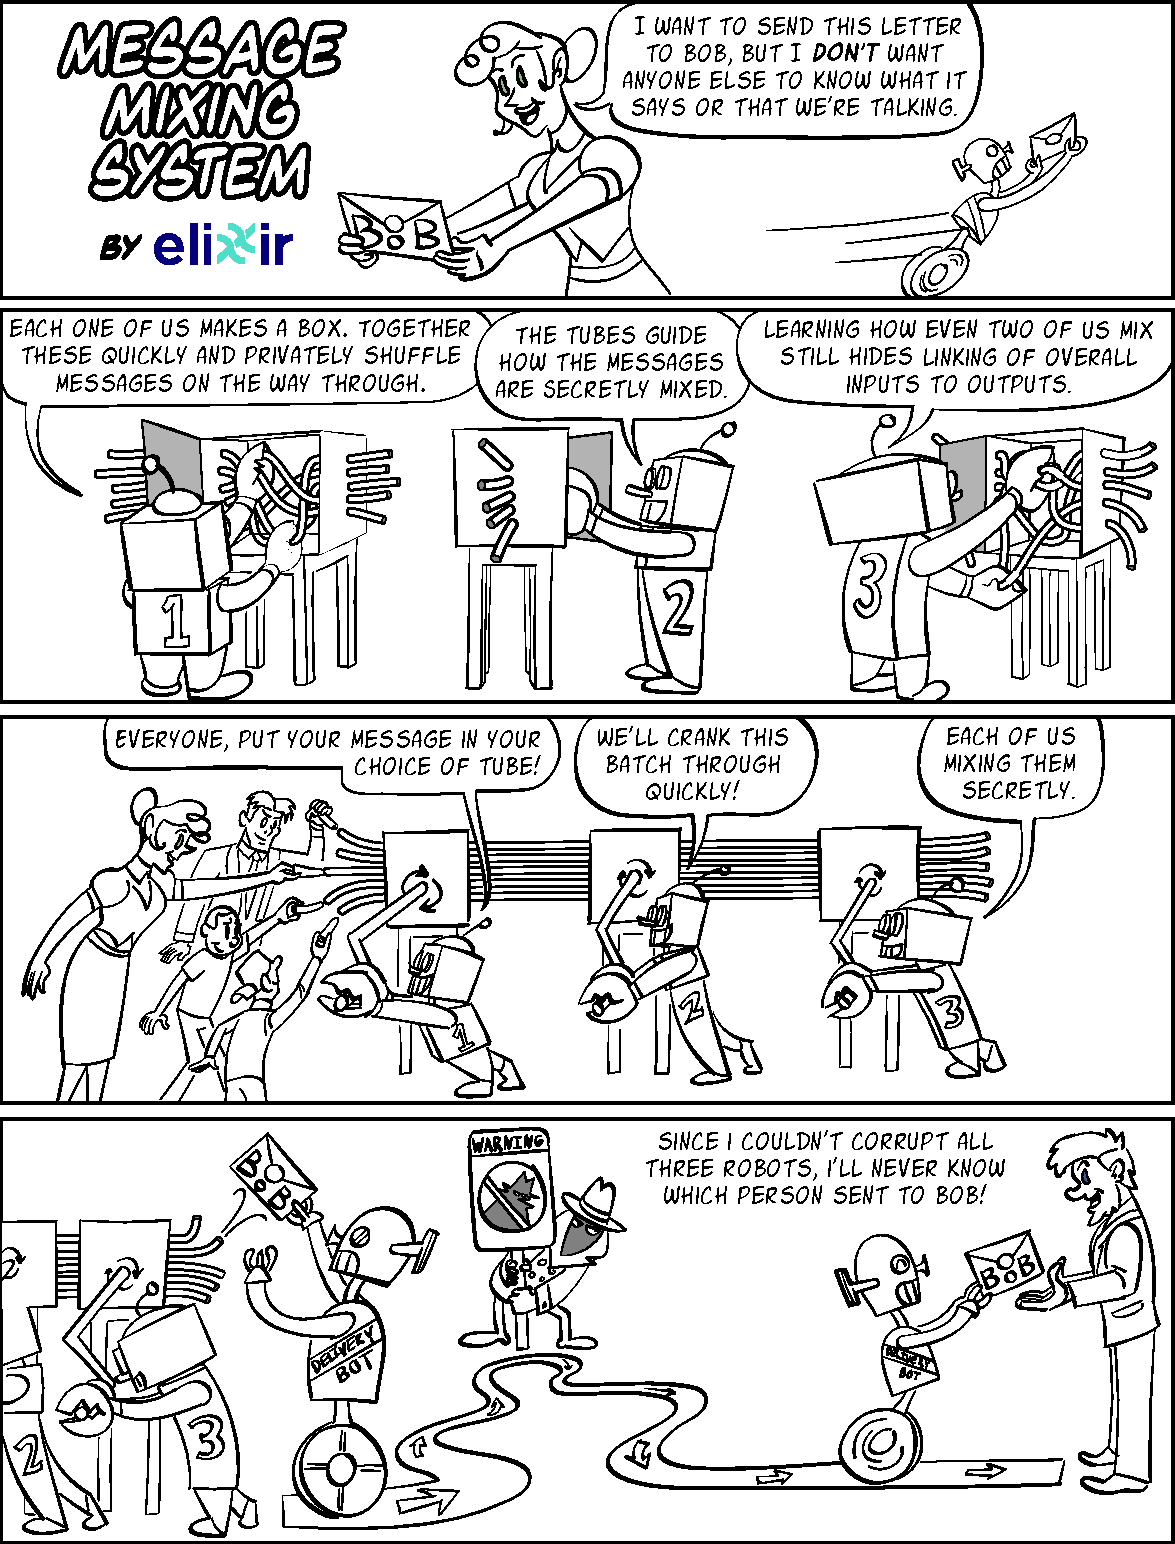
\includegraphics[width=\textwidth]{cartoons/MessageMixer.pdf}
    %\caption{Caption}
    %\label{fig:my_label}
\end{figure}

\break

Each team in the \name platform runs a single instance of a mixing network (mixnet) based on the cMix protocol~\cite{cMix}. Mixnets anonymize batches of messages and transactions, while protecting the confidentiality and integrity of each message. Besides supporting secure communications between users, these features are leveraged, and expanded to provide key functionality for the \name consensus protocol.
\iffalse
\begin{wrapfigure}{R}{0.75\textwidth}
    \centering
    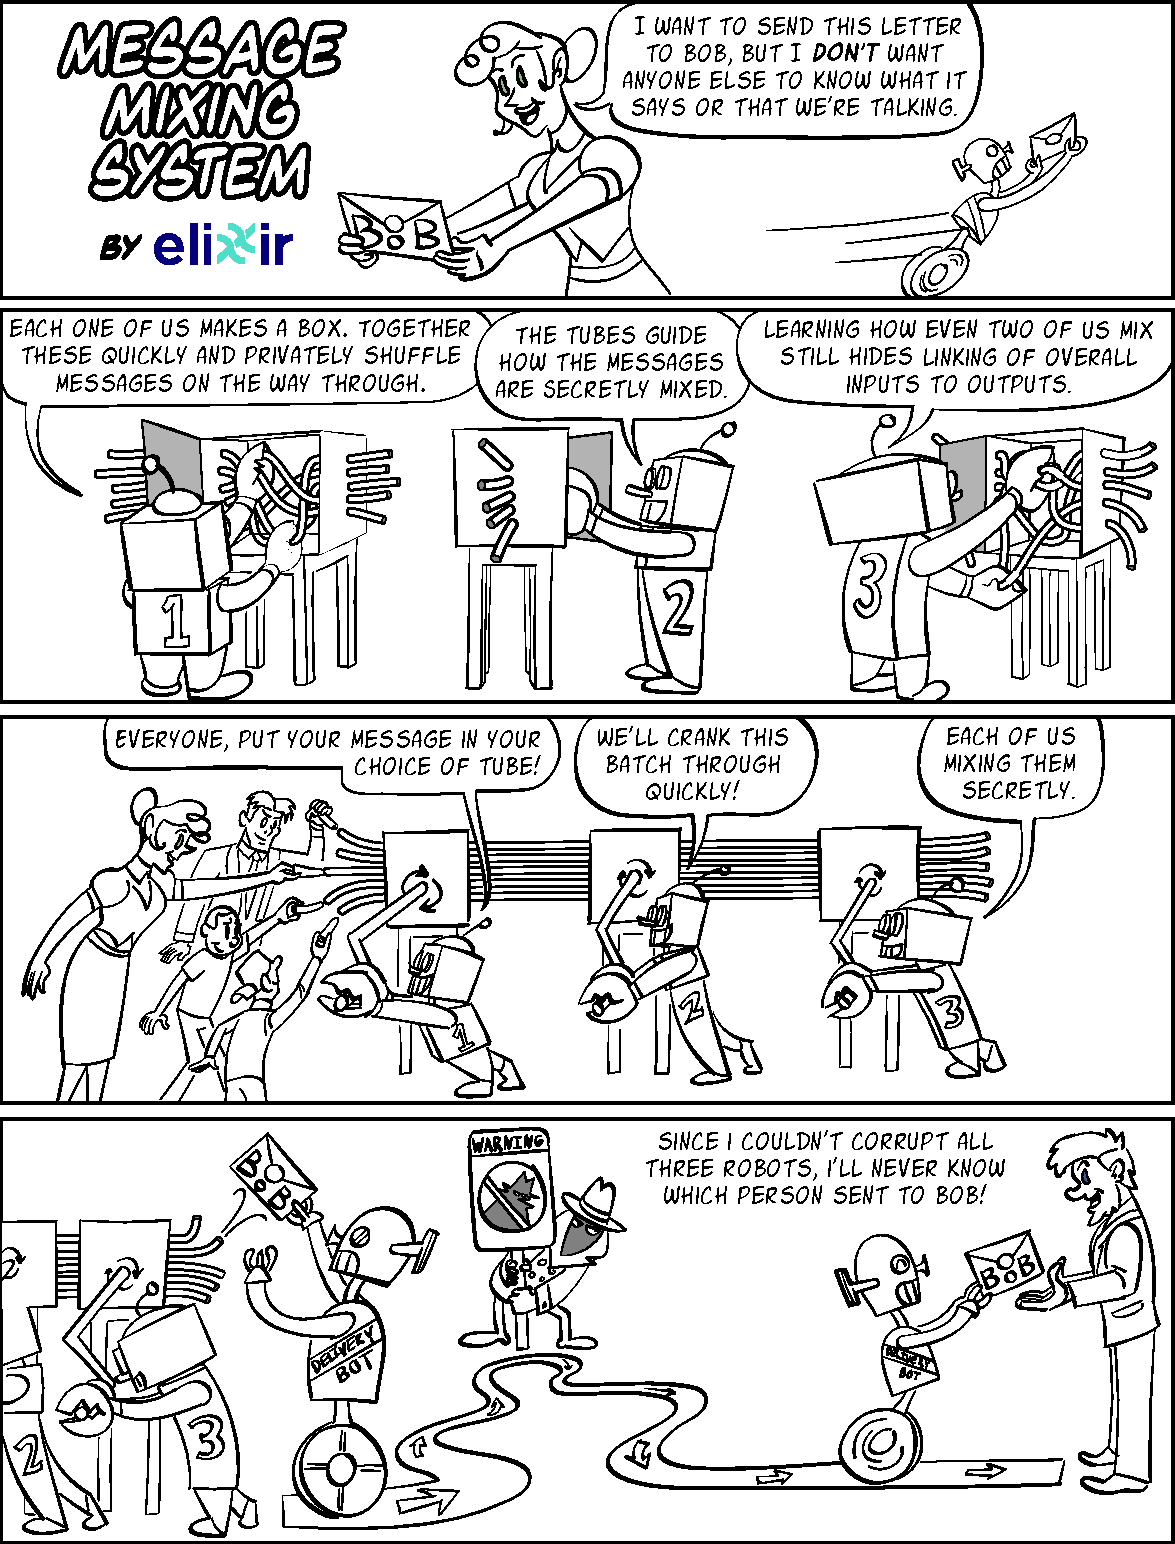
\includegraphics[width=0.74\textwidth]{cartoons/MessageMixer.png}
    %\caption{}
    %\label{}
\end{wrapfigure}
\fi

The cMix protocol is a breakthrough itself: it exhibits drastically lower real-time cryptographic latency than any other mixnet. By using a precomputation, the core cMix protocol eliminates all expensive real-time public-key operations performed on behalf of senders and recipients, and by nodes. This decreases real-time latency and lowers computational costs to clients. The core real-time phase, the second phase in the activity of a team, requires only a few quick computations, making it very well suited to applications running on lightweight clients, including chat messaging systems on smartphones, applications on low-power devices, and---most important---transaction processing.

Message processing in cMix involves 3 operations: Reception, Permutation, and Delivery. During Reception, masking network encryption is added to each already end-to-end encrypted message, while user-to-network encryption is removed from it, disassociating the senders identity from the message. In Permutation, the order of messages within a batch is shuffled, removing an observer's ability to correlate the order in which messages were received with the senders' identities. Finally, during Delivery, each node independently removes all masking network encryption, and sends the end-to-end encrypted message to its labeled destination.

The cMix Protocol has three additional important features that make it unique:

\begin{itemize}
    \item \textbf{Return Path}. The return path allows a receiver to send an immediate response through the mixnet; this permits receipts of transactions to be returned to users without the platform needing to know addressing information, thereby hiding the identity of the sender. To accomplish this goal, nodes generate additional keying material for the return path, and apply an inverse permutation so that responses arrive at the original senders.
    \item \textbf{Commitments}. Commitments are a protocol that produces data, often produced through hashing, that allows a third party to audit a computation performed by a node at a later date~\cite{commit}. All messages exchanged between nodes, the permutations they perform, and all keying materials in the mixnet's precomputation inherently function as commitments of how messages will be processed in the future, during the real-time phase of block generation. Nodes also produce a commit of the batch of encrypted messages before any decryption takes place. Commits function as an efficient mechanism for verifying that nodes perform their operations correctly.
    \item \textbf{Group Opening}. During the delivery operation, before each node in a team decrypts the batch of messages they have received, they create a commit of the batch, confirm with one another that all commits are identical, and then proceed to decrypt the batch independently. This guarantees that all nodes in the team work on the same content before any sensitive information is received. This prevents any single node from accessing sensitive information when other nodes are excluded from having the same access. This ensures that all honest nodes in the team are empowered to protect the integrity of the team and the properties they provide, namely confidentiality and anonymity.
\end{itemize}

With these features, \name provides integrity and anonymity for users sending messages and transactions through the platform. In \name, any honest node can, with non-negligible probability, identify nodes that violate integrity, and prevent malicious nodes improperly indicting an honest node. Lastly, any single honest node is able to protect user anonymity.

% Conclusion
\section{Conclusion}

\name is designed to enable true digital sovereignty for the first time by giving users the privacy and speed they expect. \name team members have built on decades of innovation in cryptographic systems---much of it their own---to create a platform that uniquely ensures the integrity and privacy of digital assets and communications. With \name, no-one can read your messages or steal your money. Period.

The \name platform protects privacy through an anonymous mixnet protocol, and a blockchain that stores tokens, not transactions. Likewise, it achieves finality quickly by abandoning the use of traditional signature-based payment processing in favor of hash-based authentications. This is achieved through the platform’s unique consensus mechanism, whereby a group of system nodes works as a team, with integrity guarantees provided via verifiable proofs. In \name, future improvements in computational power translate directly to block finality being realized more quickly, and the architecture enables linear scaling of block processing as the network grows.

\name design is unique in being able to, for the first time, scale to provide users globally with a high performing payment and messaging solution that affirms and preserves their right to digital sovereignty.


%References 
\section{References}

\printbibliography[heading=none]


\end{document}
